\documentclass[12pt, twoside]{article}
\usepackage[letterpaper, margin=1in, headsep=0.5in]{geometry}
\usepackage[english]{babel}
\usepackage[utf8]{inputenc}
\usepackage{amsmath}
\usepackage{amsfonts}
\usepackage{amssymb}
\usepackage{tikz}
\usetikzlibrary{quotes, angles}
\usepackage{graphicx}
%\usepackage{pgfplots}
%\pgfplotsset{width=10cm,compat=1.9}
%\usepgfplotslibrary{statistics}
%\usepackage{pgfplotstable}
%\usepackage{tkz-fct}
%\usepackage{venndiagram}

\usepackage{fancyhdr}
\pagestyle{fancy}
\fancyhf{}
\renewcommand{\headrulewidth}{0pt} % disable the underline of the header

\fancyhead[RE]{\thepage}
\fancyhead[RO]{\thepage \\ Name: \hspace{3cm}}
\fancyhead[L]{BECA / Dr. Huson / Geometry 10th Grade\\* Unit 3: Volume and angle bisectors \\ 
7 October 2019}

\begin{document}
\subsubsection*{3.3 Do Now: Area and volume}
  \begin{enumerate}

  \item Complete the construction of a line perpendicular to line $l$ through the point $P$. 
  \vspace{4cm}
    \begin{center}
    \begin{tikzpicture}[rotate=-20]
      \draw [<->, thick] (-2,0)--(8,0)node[below]{$l$}--(9,0);
      \draw [fill] (4,2) circle [radius=0.05] node[right]{$P$};
      %\draw [fill] (5,0) circle [radius=0.05] node[below]{$B$};
    \end{tikzpicture}
    \end{center} \vspace{4cm}
  
  \item Find the volume of a box (rectanglar prism) having a length of 11.2 centimeters, a depth of 5.5 cm, and a height of 8.3 cm. Show the calculation.
  \begin{flushright}
    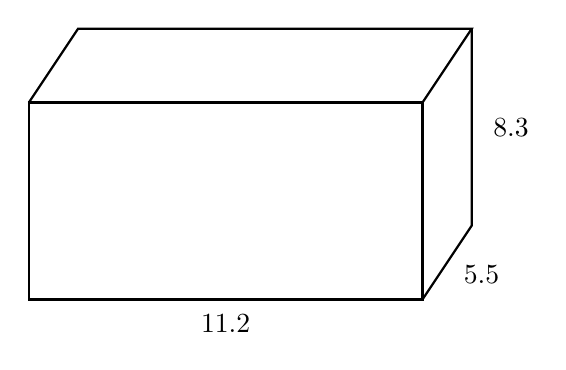
\begin{tikzpicture}[scale=1.25]
      \draw [-, thick] (0,0)--(4,0)--(4,2)--(0,2)--cycle;
      \draw [-, thick] (0,2)--(0.5,2.75)--(4.5,2.75)--(4,2);
      \draw [-, thick] (4,0)--(4.5,0.75)--(4.5,2.75);
      \node at (4.9, 1.75){$8.3$};
      \node at (2, -0.25){$11.2$};
      \node at (4.6, 0.25){$5.5$};
    \end{tikzpicture}
    \end{flushright} \vspace{2cm}

    \newpage

    \item The shape shown below is a rectangle with two triangles. Its height is 5 cm. The rectangle is 8 cm long, and each triangle has a base of 2 cm. \\[0.25cm]
    Find the total area of the shape by adding the rectangular area to the two triangle parts.
    \begin{flushright} 
    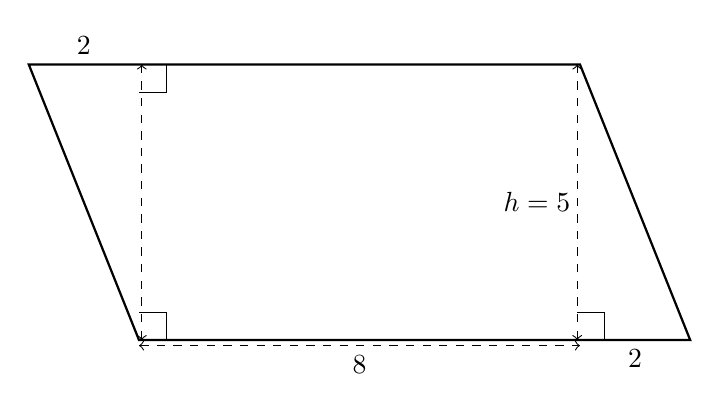
\begin{tikzpicture}[scale=0.7]
      \draw [thick]
      (0,0)--(-2,5)--(8,5)--(10,0)--cycle;
      \draw [dashed,<->] (7.95,0)--(7.95,5);
      \draw [dashed,<->] (0.05,0)--(0.05,5);
      %\draw [dashed,<->] (0,2.1)--(7,2.1);
      %\draw [->] (45:0.5)--(45:0.9142);
      %\draw [->] (45:2.3)--(45:1.9142);
      \draw (0,0)++(0,0.5)--++(0.5,0)--+(0,-0.5);
      \draw (0,5)++(0,-0.5)--++(0.5,0)--+(0,0.5);
      \draw (7.95,0)++(0,0.5)--++(0.5,0)--+(0,-0.5);
      \draw [dashed,<->] (0,-0.1)--(8,-0.1);
      \node at (4,-0.1)[below]{$8$};
      \node at (8,2.5)[left]{$h=5$};
      \node at (9,0)[below]{$2$};
      \node at (-1,5)[above]{$2$};
    \end{tikzpicture}
    \end{flushright} 
     \vspace{4cm}

\item As shown below, two lines intersect making four angles: $\angle 1$, $\angle 2$, $\angle 3$, and $\angle 4$. Given that $m\angle 2= 7x-30$ and $m\angle 3=3x+10$, find $m\angle 1$. (check your solution)
    \begin{flushright}
    \begin{tikzpicture}[scale=0.7, rotate=20]
      \draw [<->, thick] (0,-1.5)--(10,1.5);
      \draw [<->, thick] (2,2.5)--(7,-2.5);
      \node at (3,.4){1};
      \node at (6,-.6){3};
      \node at (5,1){2};
      \node at (4,-1){4};
      %\draw [fill] (0,0) circle [radius=0.05] node[below]{$P$};
      %\draw [fill] (6,0) circle [radius=0.05] node[below]{$R$};
      %\draw [fill] (3,0) circle [radius=0.05] node[below]{$Q$};
    \end{tikzpicture}
    \end{flushright} \vspace{2cm} 


\end{enumerate}
\end{document}
